% !Mode:: "TeX:UTF-8"
% !TEX program  = pdflatex
\documentclass[a4paper]{article}

% import settings, modify the number of homework in this file

\usepackage[T1]{fontenc}
\usepackage{amsmath, amssymb, amsthm}
% amsmath: equation*, amssymb: mathbb, amsthm: proof
\usepackage{moreenum}
\usepackage{mathtools}
\usepackage{url}
\usepackage{graphicx}
\usepackage{subcaption}
\usepackage{booktabs} 
\usepackage[mathcal]{eucal}
\usepackage{dsfont}
\usepackage{geometry}
\geometry{left=30mm,right=30mm,	top=42mm, bottom=33mm}

\usepackage[numbered,framed]{matlab-prettifier}
\lstset{
	style              = Matlab-editor,
	captionpos         =b,
	basicstyle         = \mlttfamily,
	escapechar         = ",
	mlshowsectionrules = true,
}

% set the homework count number
\usepackage[thehwcnt = 1]{iidef}

\newcommand\dif{\text{d}}
\newcommand\no{\noindent}
\newcommand\dis{\displaystyle}
\newcommand\ls{\leqslant}
\newcommand\gs{\geqslant}

\newcommand\limit{\dis\lim\limits}
\newcommand\limn{\dis\lim\limits_{n\to\infty}}
\newcommand\limxz{\dis\lim\limits_{x\to0}}
\newcommand\limxi{\dis\lim\limits_{x\to\infty}}
\newcommand\limxpi{\dis\lim\limits_{x\to+\infty}}
\newcommand\limxni{\dis\lim\limits_{x\to-\infty}}
\newcommand\limtpi{\dis\lim\limits_{t\to+\infty}}
\newcommand\limtni{\dis\lim\limits_{t\to-\infty}}

\newcommand\sumn{\dis\sum\limits_{n=1}^{\infty}}
\newcommand\sumnz{\dis\sum\limits_{n=0}^{\infty}}

\newcommand\sumi{\dis\sum\limits_{i=1}^{\infty}}
\newcommand\sumiz{\dis\sum\limits_{i=0}^{\infty}}
\newcommand\sumin{\dis\sum\limits_{i=1}^{n}}
\newcommand\sumizn{\dis\sum\limits_{i=0}^{n}}

\newcommand\sumk{\dis\sum\limits_{k=1}^{\infty}}
\newcommand\sumkz{\dis\sum\limits_{k=0}^{\infty}}
\newcommand\sumkn{\dis\sum\limits_{k=0}^n}
\newcommand\sumkfn{\dis\sum\limits_{k=1}^n}

\newcommand\pzx{\dis\frac{\partial z}{\partial x}}
\newcommand\pzy{\dis\frac{\partial z}{\partial y}}

\newcommand\pfx{\dis\frac{\partial f}{\partial x}}
\newcommand\pfy{\dis\frac{\partial f}{\partial y}}

\newcommand\pzxx{\dis\frac{\partial^2 z}{\partial x^2}}
\newcommand\pzxy{\dis\frac{\partial^2 z}{\partial x\partial y}}
\newcommand\pzyx{\dis\frac{\partial^2 z}{\partial y\partial x}}
\newcommand\pzyy{\dis\frac{\partial^2 z}{\partial y^2}}

\newcommand\pfxx{\dis\frac{\partial^2 f}{\partial x^2}}
\newcommand\pfxy{\dis\frac{\partial^2 f}{\partial x\partial y}}
\newcommand\pfyx{\dis\frac{\partial^2 f}{\partial y\partial x}}
\newcommand\pfyy{\dis\frac{\partial^2 f}{\partial y^2}}

\newcommand\intzi{\dis\int_{0}^{+\infty}}
\newcommand\intd{\dis\int}
\newcommand\intab{\dis\int_a^b}

\newcommand{\degree}{^\circ}

\newcommand\ma{\mathcal{A}}
\newcommand\mb{\mathcal{B}}
\newcommand\mc{\mathcal{C}}
\newcommand\me{\mathcal{E}}
\newcommand\mg{\mathcal{g}}

\newcommand\mcc{\mathbb{C}}
\newcommand\mrr{\mathbb{R}}
\newcommand\mzz{\mathbb{Z}}

\newcommand\mx{\bf{x}}
\newcommand\mX{\bf{X}}
\newcommand\my{\bf{y}}
\newcommand\mY{\bf{Y}}
%%=============================================

%%=====定义新数学符号===============================
\DeclareMathOperator{\sgn}{sgn}
\DeclareMathOperator{\arccot}{arccot}
\DeclareMathOperator{\arccosh}{arccosh}
\DeclareMathOperator{\arcsinh}{arcsinh}
\DeclareMathOperator{\arctanh}{arctanh}
\DeclareMathOperator{\arccoth}{arccoth}
\DeclareMathOperator{\grad}{\bf{grad}}
%\DeclareMathOperator{\argmax}{argmax}
%\DeclareMathOperator{\argmin}{argmin}
%\DeclareMathOperator{\diag}{diag}
\DeclareMathOperator{\csign}{csign}
%===============================================

\thecourseinstitute{Harbin Institute of Technology, ShenZhen}
\thecoursename{Operations Research}
\theterm{Fall 2019}
\hwname{Homework}

\begin{document}
\courseheader
\name{JingXuan Yang, SZ160310217}

\begin{enumerate}
  \setlength{\itemsep}{3\parskip}

% first exercise
  \item The Research and Development Division of the Progressive Company has been developing four possible new product lines. Management must now make a decision as to which of these four products actually will be produced and at what levels. Therefore, an operations research study has been requested to find the most profitable product mix.
  
  \hspace*{4ex}A substantial cost is associated with beginning the production of any product, as given in the first row of the following table. Management's objective is to find the product mix that maximizes the total profit (total net revenue minus start-up costs).
\begin{table}[h]
	\centering
	\begin{tabular}{ccccc}
		\toprule[1.5pt]
		&\multicolumn{4}{c}{Product}\\
		\cmidrule{2-5}
		&1&2&3&4\\
		\midrule
		Start-up cost&\$50000& \$40000& \$70000&\$60000\\
	    Marginal revenue&\$70& \$60& \$90&\$80\\
		\bottomrule[1.5pt]
	\end{tabular}
\end{table}

\hspace*{4ex}Let the continuous decision variables $x_1, x_2, x_3$, and $x_4$ be the production levels of products 1, 2, 3, and 4, respectively. Management has imposed the following policy constraints on these variables:

1. No more than two of the products can be produced.

2. Either product 3 or 4 can be produced only if either product 1 or 2 is produced.

3. Either $$5x_1+3x_2+6x_3+4x_4\ls 6000$$ or $$4x_1+6x_2+3x_3+5x_4\ls 6000$$

\hspace*{4ex}Introduce auxiliary binary variables to formulate a mixed BIP model for this problem.

\begin{solution}
	
	To deal with requirement 1 and 2, we introduce four auxiliary binary variables ($y_1,y_2,y_3,y_4$) with the interpretation
	\begin{equation*}
	y_j=\left\{\begin{aligned}
	&1,\quad\text{if } x_j>0 \text{ can hold} \\
	&0,\quad\text{if } x_j=0 \text{ must hold} \\
	\end{aligned}\right. 
	\end{equation*}
	for $j=1,2,3,4.$ To enforce this interpretation in the model, we add the constraints:
	\begin{equation*}
	\begin{aligned}
	x_j&\ls My_j,\ j=1,2,3,4\\
	y_1+y_2+y_3+y_4&\ls 2\\
	y_3&\ls y_1+y_2\\
	y_4&\ls y_1+y_2\\
	y_j&\text{ is binary},\ j=1,2,3,4
	\end{aligned}
	\end{equation*}
	
	To deal with requirement 3, we introduce another auxiliary binary variable $y_5$ with the interpretation
	\begin{equation*}
	y_5=\left\{\begin{aligned}
	&1,\quad\text{if } 4x_1+6x_2+3x_3+5x_4\ls 6000 \text{ must hold} \\
	&0,\quad\text{if } 5x_1+3x_2+6x_3+4x_4\ls 6000 \text{ must hold} \\
	\end{aligned}\right. 
	\end{equation*}
	With the help of an extremely large positive number $M$, this interpretation is enforced by adding the constraints:
	\begin{equation*}
	\begin{aligned}
		5x_1+3x_2+6x_3+4x_4&\ls 6000+My_5\\
		4x_1+6x_2+3x_3+5x_4&\ls 6000+M(1-y_5)\\
		y_5 &\text{ is binary}
	\end{aligned}
	\end{equation*}
	Consequently, after we move all variables to the left-hand side of the constraints, the complete model is
	
	Maximize $$Z=70x_1-50000y_1+60x_2-40000y_2+90x_3-70000y_3+80x_4-60000y_4$$
	subject to
	\begin{equation*}
	\begin{aligned}
	x_j-My_j&\ls 0,\ j=1,2,3,4\\
	y_1+y_2+y_3+y_4&\ls 2\\
	-y_1-y_2+y_3&\ls 0\\
	-y_1-y_2+y_4&\ls 0\\
	5x_1+3x_2+6x_3+4x_4-My_5&\ls 6000\\
	4x_1+6x_2+3x_3+5x_4+My_5&\ls 6000+M\\
	x_1,x_2,x_3,x_4&\gs 0\\
	y_j \text{ is binary},\ j&=1,2,3,4,5
	\end{aligned}
	\end{equation*}
\end{solution}

% second esercise
\item An increasing number of Americans are moving to a warmer climate when they retire. To take advantage of this trend, Sunny Skies Unlimited is undertaking a major real estate development project. The project is to develop a completely new retirement community (to be called Pilgrim Haven) that will cover several square miles. One of the decisions to be made is where to locate the two fire stations that have been allocated to the community. For planning purposes, Pilgrim Haven has been divided into five tracts, with no more than one fire station to be located in any given tract. Each station is to respond to all the fires that occur in the tract in which it is located as well as in the other tracts that are assigned to this station. Thus, the decisions to be made consist of (1) the tracts to receive a fire station and (2) the assignment of each of the other tracts to one of the fire stations. The objective is to minimize the overall average of the \textit{response times} to fires.

\hspace*{4ex}The following table gives the average response time to a fire in each tract (the columns) if that tract is served by a station in a given tract (the rows). The bottom row gives the forecasted average number of fires that will occur in each of the tracts per day.

\begin{table}[h]
	\centering
	\begin{tabular}{cccccc}
		\toprule[1.5pt]
		&\multicolumn{5}{c}{Response Times (in minutes)}\\
		&\multicolumn{5}{c}{Fire in Tract}\\
		\cmidrule{2-6}
		Assigned Station&1&2&3&4&5\\
		\midrule
		1&5&12& 30&20&15\\
		2&20&4& 15&10&25\\
		3&15&20& 6&15&12\\
		4&25&15& 25&4&10\\
		5&10&25& 15&12&5\\
		\midrule
		Average Frequency&2 per day&1 per day&3 per day&1 per day&3 per day\\
		\bottomrule[1.5pt]
	\end{tabular}
\end{table}

Formulate a BIP model for this problem. Identify any constraints that correspond to mutually exclusive alternatives or contingent decisions.

\begin{solution}
	
	First define decision variables as follows:
	\begin{equation*}
	x_{ij}=\left\{\begin{aligned}
	&1,\quad \text{if tract } j \text{ is served by tract } i\\
	&0,\quad \text{otherwise}
	\end{aligned}\right.
	\end{equation*}
	for $i,j=1,2,\cdots,5.$
	
	Requirement 1: two fire stations should be allocated to two of the five tracts,
	$$ \sum_{i=1}^{5} x_{ii}=2, $$
	which is a mutually exclusive alternative.
	
	Requirement 2: only a tract with a station can serve other tracts,
	$$x_{ij}\ls x_{ii}, \ i,j=1,2,\cdots,5,$$
	which is a contingent decision.
	
	Requirement 3: a tract can be served by only one station,
	$$\sum_{i=1}^{5}x_{ij}=1,\ j=1,2,\cdots,5,$$
	which is a mutually exclusive alternative.
	
	\hspace*{4ex}Let $t_{ij}$ be the response time to a fire in tract $j$ if that tract is served by a station in tract $i$, and $f_j$ be the forecasted average number of fires that will occur in tract $j$ per day. Then the BIP model can be formulated as follows:
	
	Minimize $$Z=\sum_{i=1}^{5}\sum_{j=1}^{5}f_j\cdot t_{ij}\cdot x_{ij}$$
	subject to
	\begin{equation*}
	\begin{aligned}
	\sum_{i=1}^{5} x_{ii}&=2\\
	x_{ij}&\ls x_{ii},\ i,j=1,2,\cdots,5\\
	\sum_{i=1}^{5}x_{ij}&=1,\ j=1,2,\cdots,5\\
	x_{ij} &\text{ is binary},\ i,j=1,2,\cdots,5\\
	\end{aligned}
	\end{equation*}
	
\end{solution}

\item Consider the following IP problem.

Minimize $$Z=2x_1+3x_2$$
subject to
\begin{equation*}
\begin{aligned}
x_1+x_2&\gs 3\\
x_1+3x_2&\gs 6\\
x_1,x_2&\gs 0\\
x_1,x_2&\text{ are integers}
\end{aligned}
\end{equation*}
Use the MIP branch-and-bound algorithm presented in Topic 6 Part (II) Section 3 to solve this problem by hand. For each subproblem, solve its LP relaxation graphically. (Hint: This problem is a minimization problem.)
\begin{solution}
	
	 \textbf{Initialization.}\quad Since this is a minimization problem, we set $Z^*=+\infty$. Form the LP relaxation of this problem by deleting the set of constraints that $x_1$ and $x_2$ are integers. Solve this LP relaxation problem graphically, we obtain
	\begin{equation*}
	\text{LP relaxation of the whole problem: } (x_1,x_2)=\left(\dfrac{3}{2},\dfrac{3}{2}\right),\ \text{with } Z=\dfrac{15}{2}.
	\end{equation*}
	Because it has feasible solutions and this optimal solution has noninteger values for its integer-restricted variables, the whole problem is not fathomed, so the algorithm continues with the full iteration below.
	
	\textbf{Iteration 1.}\quad In this optimal solution for the LP relaxation, the first integer-restricted variable that has a noninteger value is $x_1=\tfrac{3}{2}$, so $x_1$ becomes the branching variable. Branching from All node (all feasible solution) with this branching variable the creates the following two subproblems:
	
	\textit{Subproblem 1}:
	
	Original problem plus additional constraint $$x_1\ls 1.$$
	
	\textit{Subproblem 2}:
	
	Original problem plus additional constraint $$x_1\gs 2.$$
	
	Deleting the integer constraints again and solving the resulting LP relaxations of these two subproblem graphically yield the following results.
	
	\textit{Subproblem 1}:
	
	\hspace*{4ex}Optimal solution for LP relaxation: $(x_1,x_2)=(1,2 )$, with $Z^*=8.$
	
	\textit{Subproblem 2}:
	
	\hspace*{4ex}Optimal solution for LP relaxation: $(x_1,x_2)=\left( 2,\dfrac{4}{3}\right) $, with $Z=8.$
	
	\hspace*{4ex}Bound: $Z\gs Z^*=8.$
	
	\hspace*{4ex}These outcomes mean that subproblem 1 is fathomed by test 3 and subproblem 2 is fathomed by test 1. Then there are no remaining subproblems, so the current incumbent is optimal.
	\begin{equation*}
	\text{Optimal solution}=(1,2),\ \text{with } Z=8.
	\end{equation*}
	
	\hspace*{4ex}These results are summarized by the branching tree given in Fig.\ref{f1}.
	
	\begin{figure}[htbp]
		\centering
		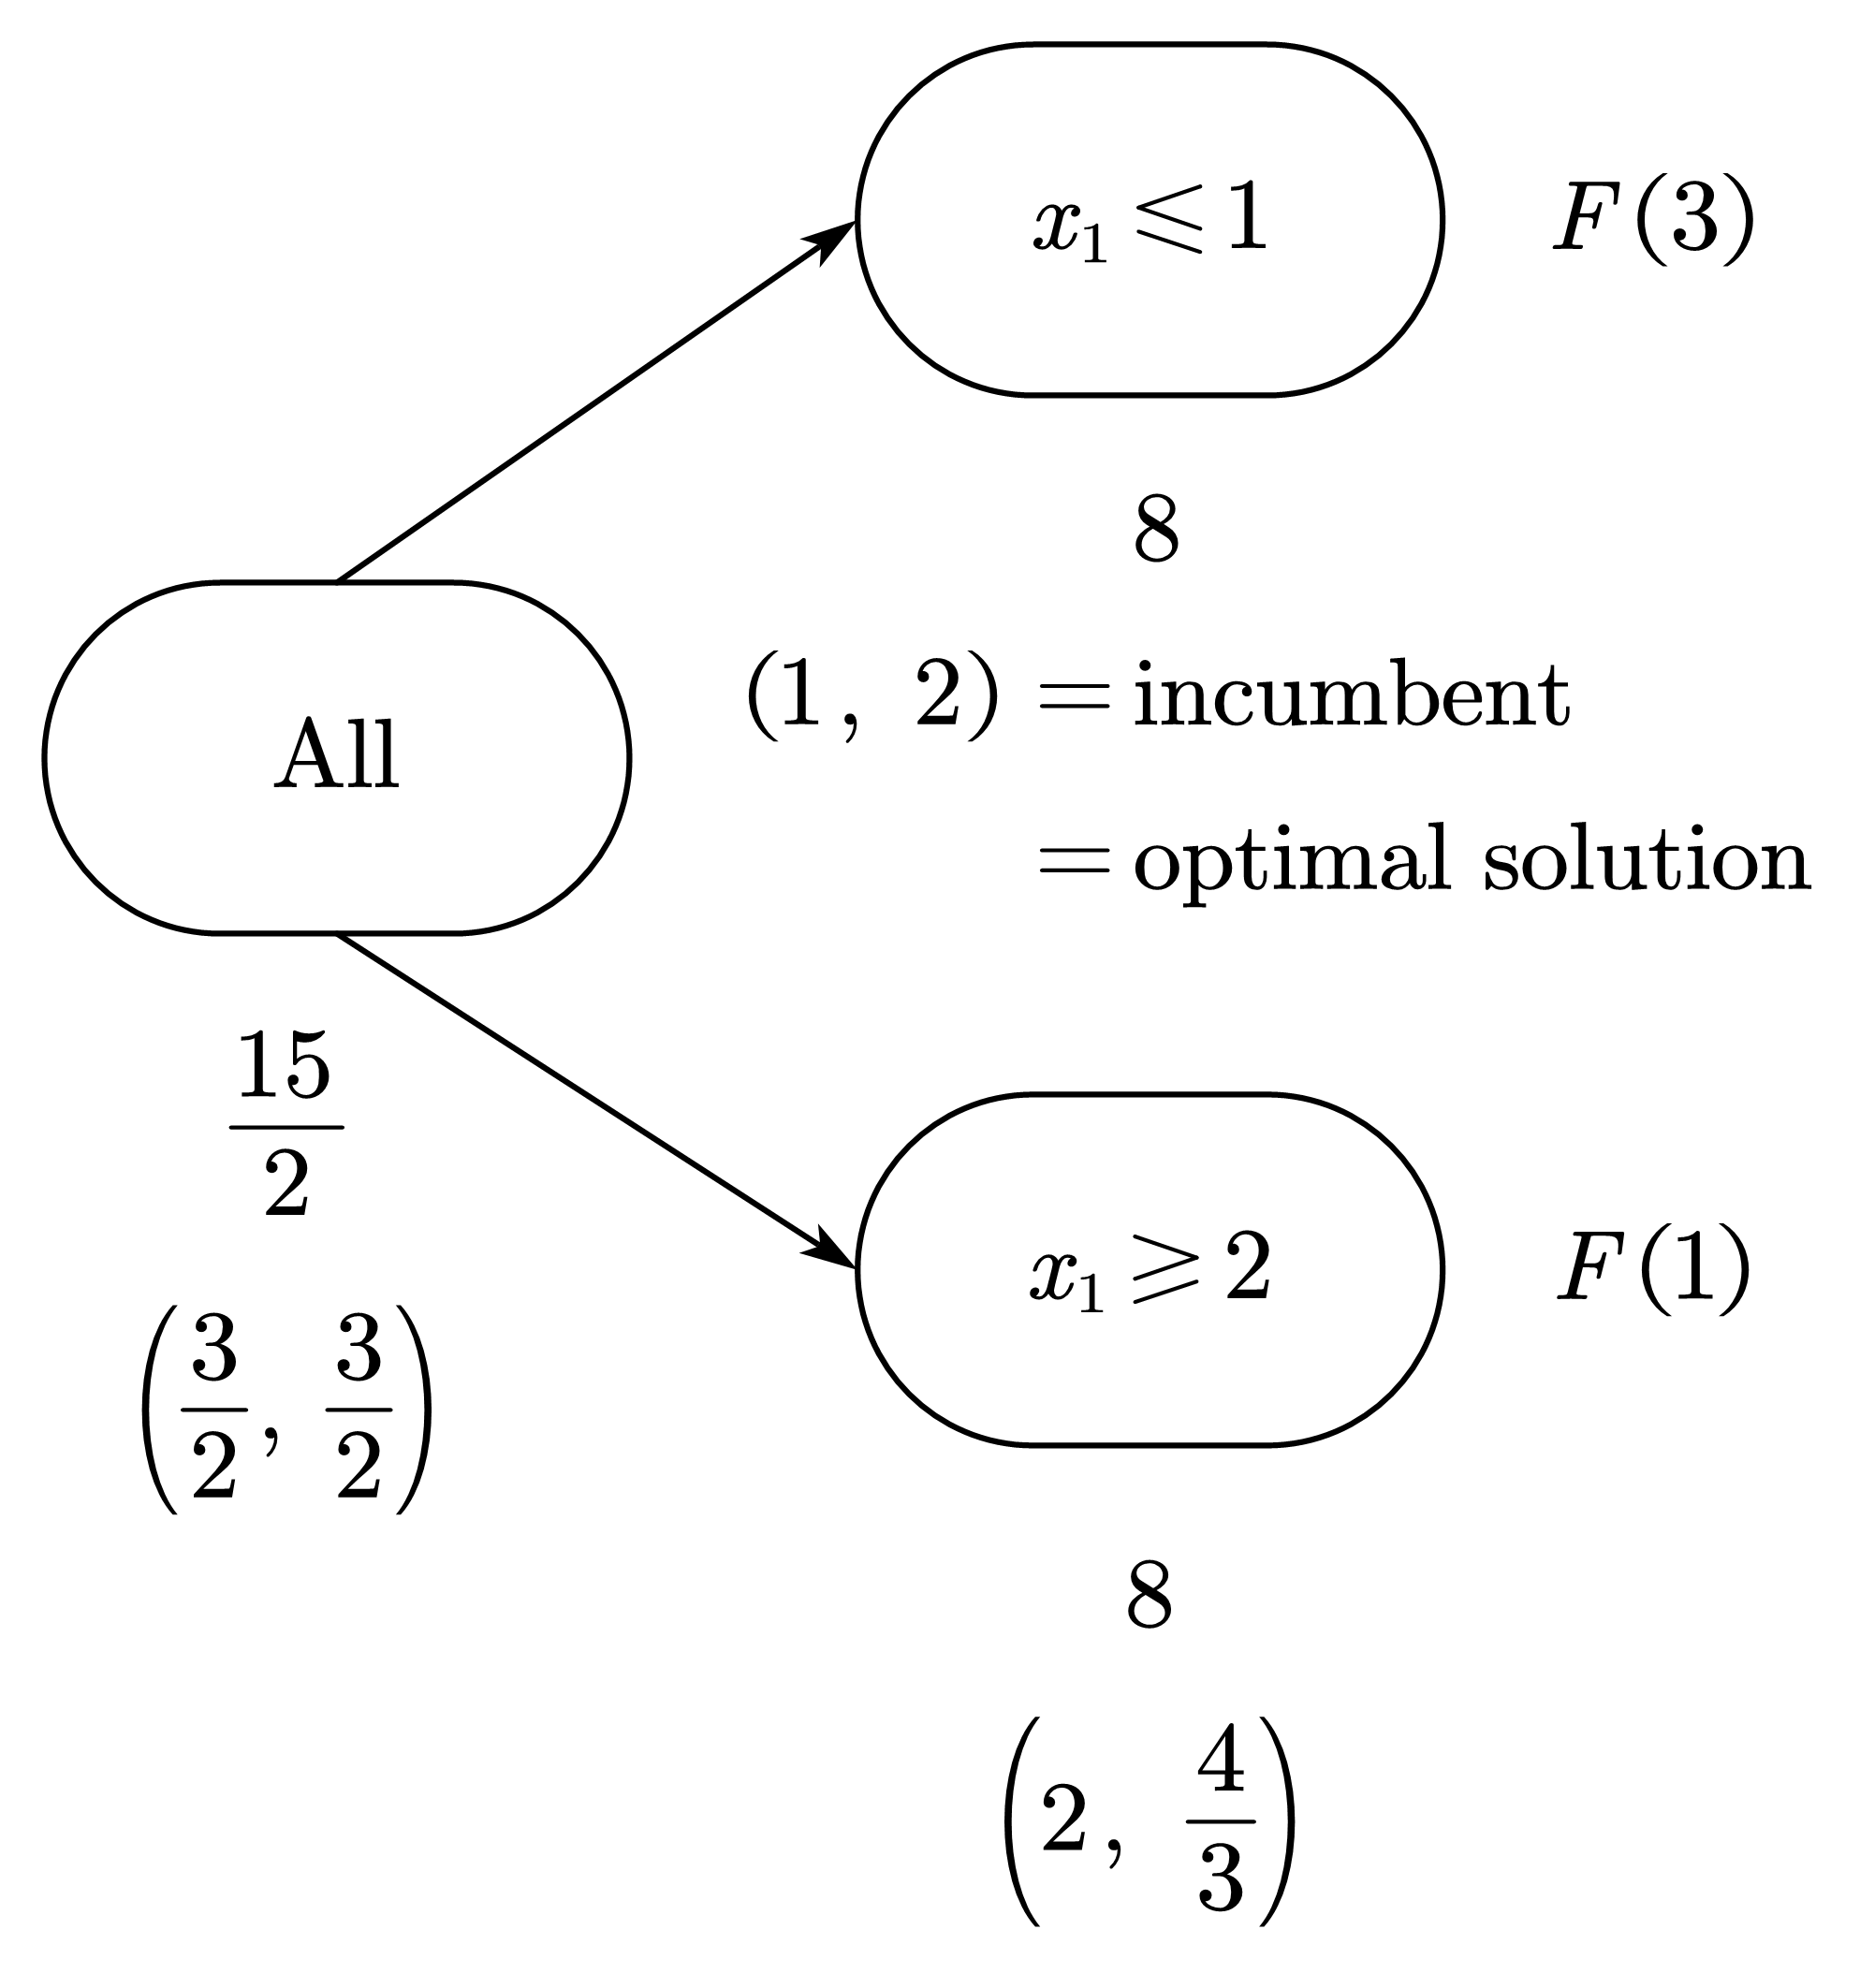
\includegraphics[width = 0.4\textwidth]{f1}
		\caption{The branching tree for this IP problem}
		\label{f1}
	\end{figure}
	
\end{solution}
\vspace*{-1cm}

\item Use the following set of constraints for the same pure BIP problem to fix as many variables as possible. Also identify the constraints which become redundant because of the fixed variables.
\begin{equation*}
\begin{aligned}
3x_3-x_5+x_7&\ls 1\qquad(1)\\
x_2+x_4+x_6&\ls 1\qquad(2)\\
x_1-2x_5+2x_6&\gs 2\qquad(3)\\
x_1+x_2-x_4&\ls 0\qquad(4)\\
\end{aligned}
\end{equation*}

\begin{solution}
	
	From Eq.(1), since $3(1)-(1)+(0)=2>1$, we see that $x_3=0$, then Eq.(1) is redundant since $-(0)+(1)\ls 1$. From Eq.(3), since $  (1)-2(1)+2(1)=1<2$ and $(1)-2(0)+2(0)=1<2$, we see that $x_5=0, x_6=1$. What's more, from Eq.(2), since $x_6=1$, then $x_2=x_4=0$, thus from Eq.(4), $x_1=0$. Then all variables are fixed except $x_7$ and all four equations become redundant, thus the solution is $(0,0,0,0,0,1,x_7)$.
	
\end{solution}
\vspace*{-0.5cm}

\item Apply the procedure for tightening constraints to the following constraint for a pure BIP problem: $$3x_1-2x_2+x_3\ls 3.$$

\begin{solution}
	
	The constraint is $$3x_1-2x_2+x_3\ls 3\quad (a_1=3,a_2=-2,a_3=1,b=3).$$
	
	\begin{enumerate}
		\item $S=3+1=4$.
		\item $a_1=3$ satisfies $S<b+|a_1|$, since $4<3+3=6$. Also $a_2=-2$ satisfies $S<b+|a_2|$, since $4<3+2=5$. Choose $a_1$ arbitrarily. 
		\item $\bar{a}_1=S-b=4-3=1$ and $\bar{b}=S-|a_1|=4-3=1$. The new tighter constraint is $$x_1-2x_2+x_3\ls 1\quad(a_1=1,a_2=-2,a_3=1,b=1).$$
	\end{enumerate}

	\begin{enumerate}
		\item $S=1+1=2$.
		\item $a_2=-2$ satisfies $S<b+|a_2|$, since $2<1+2=3$. 
		\item Increase $a_2$ to $b-S=-1$ The new tighter constraint is $$x_1-x_2+x_3\ls 1\quad(a_1=1,a_2=-1,a_3=1,b=1).$$
	\end{enumerate}
	
	\begin{enumerate}
		\item $S=1+1=2$.
		\item No $a_j\neq 0$ satisfies $S<b+|a_j|$, so stop; $x_1-x_2+x_3\ls 1$ is the desired tightened constraint.
	\end{enumerate}
	
\end{solution}

\item One of the constraints of a certain pure BIP problem is $$x_1+3x_2+2x_3+4x_4\ls 5$$
Identify all the minimal covers for this constraint, and then give the corresponding cutting planes.

\begin{solution}
	The minimal covers and corresponding cutting planes are shown in Tab.\ref{tabminimal}.
	\begin{table}[H]
		\centering
		\caption{Minimal covers and corresponding cutting planes}
		\label{tabminimal}
		\begin{tabular}{ccc}
			\toprule[1.5pt]			
			Number&Minimal Cover&Cutting Plane\\
			\midrule
			1&$\{x_3,x_4\}$              &$x_3+x_4\ls 1$\\
			2&$\{x_2,x_4\}$              &$x_2+x_4\ls 1$\\
			3&$\{x_1,x_2,x_3\}$              &$x_1+x_2+x_3\ls 2$\\
			\bottomrule[1.5pt]
		\end{tabular}
	\end{table}
	
\end{solution}

% w.r.t the external
\end{enumerate}
%  The source code to plot Figure \ref{fig:1} could be found in Appendix \ref{sec:a:code}. Here are the core codes:
%  \lstinputlisting[firstline=6,lastline=7, firstnumber=6]{matlabscript.m}

%  \newpage
%  \appendix
%  \section{Source code}
%  \label{sec:a:code}
%  % \lstlistoflistings
%  Source code for plotting Figure \ref{fig:1} is shown as follows.
%  \lstinputlisting[caption=FigurePlot]{matlabscript.m}
  
\end{document}
